В информационный центр приходят клиенты через интервал времени 10 $\pm$ 2 минуты. Если все три имеющихся оператора заняты, клиенту отказывают в обслуживании. 

Операторы имеют разную производительность и могут обеспечивать обслуживание среднего запроса пользователя за 20 $\pm$ 5; 40 $\pm$ 10; 40 $\pm$ 20. 

Клиенты стремятся занять свободного оператора с максимальной производительностью. 

Полученные запросы сдаются в накопитель. Откуда выбираются на обработку. На первый компьютер запросы от 1 и 2-ого операторов, на второй – запросы от 3-его. Время обработки запросов первым и 2-м компьютером равны соответственно 15 и 30 мин. Промоделировать процесс обработки 300 запросов.

Использовать язык GPSS.

\begin{figure}[h]
	\begin{center}
		{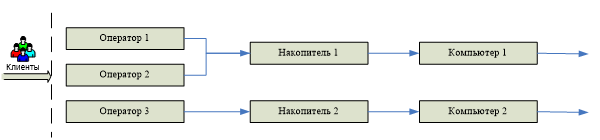
\includegraphics[scale = 0.9]{img/schema.png}}
		\caption{Общая схема}
		\label{fig1:image}
	\end{center}
\end{figure}